\documentclass[aspectratio=169]{beamer}

% The  following themes, you can uncomment it to use
% Want to figure out  what theme you have  on your computer(this refers to linux distro) that you can use
% the following cpmmand may help you:
%
% ls /usr/share/texlive/texmf-dist/tex/latex/beamer | grep "^beamertheme"
%
% Or you can go to:
% https://deic.uab.cat/~iblanes/beamer_gallery/   to see more info

%%%%%%%%%%%%%%%%%%%%%%%%%%%%%%%%%%%%%%%%
% \usetheme[named=mygreen]{Berkeley}
% \usetheme{Warsaw}
 \usetheme{metropolis} % reference:https://mirror.mwt.me/ctan/macros/latex/contrib/beamer-contrib/themes/metropolis/doc/metropolistheme.pdf
% \usetheme{AnnArbor}
% \usetheme{Berlin}
% \usecolortheme{crane}
% \usecolortheme{seahorse}
% \usecolortheme{dolphin}
%%%%%%%%%%%%%%%%%%%%%%%%%%%%%%%%%%%%%%%%

%%%%%%%%%%%%%%%%%%%%%%%%%%%%%%%%%%%%%%%%
% User defined color 
% you can also get more from http://latexcolor.com/
%%%%%%%%%%%%%%%%%%%%%%%%%%%%%%%%%%%%%%%%
\definecolor{mygreen}{rgb}{.125, .5, .25}


%%%%%%%%%%%%%%%%%%%%%%%%%%%%%%%%%%%%%%%%
% support for chinese
%%%%%%%%%%%%%%%%%%%%%%%%%%%%%%%%%%%%%%%%
\usepackage{ctex}

%%%%%%%%%%%%%%%%%%%%%%%%%%%%%%%%%%%%%%%%
% support for images and set the image path
%%%%%%%%%%%%%%%%%%%%%%%%%%%%%%%%%%%%%%%%
\usepackage{graphicx}
\graphicspath{ {./images/} }


%%%%%%%%%%%%%%%%%%%%%%%%%%%%%%%%%%%%%%%%
% support for table
%%%%%%%%%%%%%%%%%%%%%%%%%%%%%%%%%%%%%%%%
\usepackage{multirow}



\begin{document}
%
% Basic Information Of This Silde
%

\title{法律}
\author{法律}
\institute{法律}
\date{\today}

%%%%%%%%%%%%%%%%%%%%%%%%%%%%%%%%%%%%%%%%
% titlepage
%%%%%%%%%%%%%%%%%%%%%%%%%%%%%%%%%%%%%%%%
\begin{frame}
\titlepage
\end{frame}


%%%%%%%%%%%%%%%%%%%%%%%%%%%%%%%%%%%%%%%%
% A frame
%%%%%%%%%%%%%%%%%%%%%%%%%%%%%%%%%%%%%%%%
\begin{frame}[t]{刑法}
    违法不一定犯罪\\
    犯罪一定违法\\

    
\includegraphics[scale=0.5]{criminal_law_intro}\\ 
\end{frame}


%%%%%%%%%%%%%%%%%%%%%%%%%%%%%%%%%%%%%%%%
% A frame
%%%%%%%%%%%%%%%%%%%%%%%%%%%%%%%%%%%%%%%%
\begin{frame}[t]{刑法}
    真题:\\
    
\includegraphics[scale=0.4]{criminal_law_001}\\ 
\end{frame}

%%%%%%%%%%%%%%%%%%%%%%%%%%%%%%%%%%%%%%%%
% A frame
%%%%%%%%%%%%%%%%%%%%%%%%%%%%%%%%%%%%%%%%
\begin{frame}[t]{刑法}
    真题:\\
    
\includegraphics[scale=0.4]{criminal_law_001}\\ 
    答案:\textbf{A,盗窃别抓,坦白抢劫犯罪, 是自首行为, 自首:1 投案自首 2 交代新罪()}\\
    答案:\textbf{X, 死刑包括:1 死缓 2 死立执}\\
\end{frame}

%%%%%%%%%%%%%%%%%%%%%%%%%%%%%%%%%%%%%%%%
% A frame
%%%%%%%%%%%%%%%%%%%%%%%%%%%%%%%%%%%%%%%%
\begin{frame}[t]{刑法}
    真题:\\
    
\includegraphics[scale=0.4]{criminal_law_002}\\ 
\end{frame}

%%%%%%%%%%%%%%%%%%%%%%%%%%%%%%%%%%%%%%%%
% A frame
%%%%%%%%%%%%%%%%%%%%%%%%%%%%%%%%%%%%%%%%
\begin{frame}[t]{刑法}
    真题:\\
    
\includegraphics[scale=0.25]{criminal_law_002A}\\ 
    答案:\textbf{B, 犯罪未遂}\\
犯罪预备: 主观原因导致停止, 犯罪在\textbf{准备}阶段\\
犯罪未遂: 主观原因导致停止, 犯罪在\textbf{实施}阶段\\
犯罪中止: 客观观原因导致停止 \\
犯罪既遂:目的已经达成 \\
\end{frame}



%%%%%%%%%%%%%%%%%%%%%%%%%%%%%%%%%%%%%%%%
% A frame
%%%%%%%%%%%%%%%%%%%%%%%%%%%%%%%%%%%%%%%%
\begin{frame}[t]{刑法}
    
\includegraphics[scale=0.4]{criminal_law_basic}\\ 
    法律规定是犯罪,法律没有规定不是犯罪\\
    适用法律,人人平等\\
\end{frame}



%%%%%%%%%%%%%%%%%%%%%%%%%%%%%%%%%%%%%%%%
% A frame
%%%%%%%%%%%%%%%%%%%%%%%%%%%%%%%%%%%%%%%%
\begin{frame}[t]{刑法}
    
\includegraphics[scale=0.4]{criminal_law_range}\\ 
\end{frame}


%%%%%%%%%%%%%%%%%%%%%%%%%%%%%%%%%%%%%%%%
% A frame
%%%%%%%%%%%%%%%%%%%%%%%%%%%%%%%%%%%%%%%%
\begin{frame}[t]{刑法}
    真题:\\
    
\includegraphics[scale=0.4]{criminal_law_003}\\ 
\end{frame}


%%%%%%%%%%%%%%%%%%%%%%%%%%%%%%%%%%%%%%%%
% A frame
%%%%%%%%%%%%%%%%%%%%%%%%%%%%%%%%%%%%%%%%
\begin{frame}[t]{刑法}
    真题:\\
    
\includegraphics[scale=0.4]{criminal_law_003A}\\ 

    答案:\textbf{A, 属地原则}\\
\end{frame}



%%%%%%%%%%%%%%%%%%%%%%%%%%%%%%%%%%%%%%%%
% A frame
%%%%%%%%%%%%%%%%%%%%%%%%%%%%%%%%%%%%%%%%
\begin{frame}[t]{刑法}
    
\includegraphics[scale=0.4]{criminal_concecpt}\\ 
\end{frame}


%%%%%%%%%%%%%%%%%%%%%%%%%%%%%%%%%%%%%%%%
% A frame
%%%%%%%%%%%%%%%%%%%%%%%%%%%%%%%%%%%%%%%%
\begin{frame}[t]{刑法}
    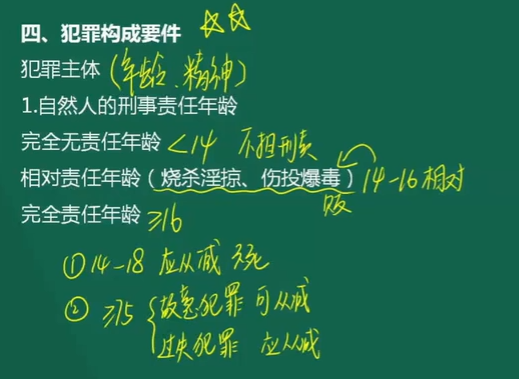
\includegraphics[scale=0.4]{criminal_element}\\ 
\end{frame}



%%%%%%%%%%%%%%%%%%%%%%%%%%%%%%%%%%%%%%%%
% A frame
%%%%%%%%%%%%%%%%%%%%%%%%%%%%%%%%%%%%%%%%
\begin{frame}[t]{刑法}
    
\includegraphics[scale=0.4]{criminal_entity}\\ 
\end{frame}




%%%%%%%%%%%%%%%%%%%%%%%%%%%%%%%%%%%%%%%%
% A frame
%%%%%%%%%%%%%%%%%%%%%%%%%%%%%%%%%%%%%%%%
\begin{frame}[t]{刑法}
    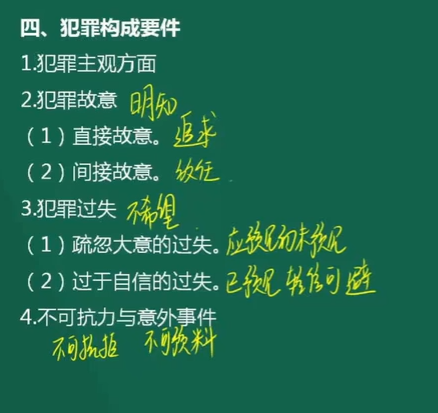
\includegraphics[scale=0.4]{criminal_host}\\ 
\end{frame}




%%%%%%%%%%%%%%%%%%%%%%%%%%%%%%%%%%%%%%%%
% A frame
%%%%%%%%%%%%%%%%%%%%%%%%%%%%%%%%%%%%%%%%
\begin{frame}[t]{刑法}
    
\includegraphics[scale=0.4]{criminal_guest}\\ 
\end{frame}



%%%%%%%%%%%%%%%%%%%%%%%%%%%%%%%%%%%%%%%%
% A frame
%%%%%%%%%%%%%%%%%%%%%%%%%%%%%%%%%%%%%%%%
\begin{frame}[t]{刑法}
    
\includegraphics[scale=0.4]{criminal_action_result}\\ 
\end{frame}



%%%%%%%%%%%%%%%%%%%%%%%%%%%%%%%%%%%%%%%%
% A frame
%%%%%%%%%%%%%%%%%%%%%%%%%%%%%%%%%%%%%%%%
\begin{frame}[t]{刑法}
    真题:\\
    
\includegraphics[scale=0.4]{criminal_law_005}\\ 
    答案:\textbf{A, 14——16 相对责任  烧杀淫掠,伤(重伤)投爆毒}\\
\end{frame}



%%%%%%%%%%%%%%%%%%%%%%%%%%%%%%%%%%%%%%%%
% A frame
%%%%%%%%%%%%%%%%%%%%%%%%%%%%%%%%%%%%%%%%
\begin{frame}[t]{刑法}
    
\includegraphics[scale=0.6]{self-defince}\\ 
\end{frame}

%%%%%%%%%%%%%%%%%%%%%%%%%%%%%%%%%%%%%%%%
% A frame
%%%%%%%%%%%%%%%%%%%%%%%%%%%%%%%%%%%%%%%%
\begin{frame}[t]{刑法}
    真题:\\
    
\includegraphics[scale=0.6]{self-defince-question}\\ 
    答案:\textbf{D, 正当防卫可以是 保护本人 他人 第三人}\\
\end{frame}


%%%%%%%%%%%%%%%%%%%%%%%%%%%%%%%%%%%%%%%%
% A frame
%%%%%%%%%%%%%%%%%%%%%%%%%%%%%%%%%%%%%%%%
\begin{frame}[t]{刑法}
    
\includegraphics[scale=0.6]{emergyce-avoiding}\\ 
\end{frame}


%%%%%%%%%%%%%%%%%%%%%%%%%%%%%%%%%%%%%%%%
% A frame
%%%%%%%%%%%%%%%%%%%%%%%%%%%%%%%%%%%%%%%%
\begin{frame}[t]{刑法}
    
\includegraphics[scale=0.6]{criminal_status}\\ 
\end{frame}


%%%%%%%%%%%%%%%%%%%%%%%%%%%%%%%%%%%%%%%%
% A frame
%%%%%%%%%%%%%%%%%%%%%%%%%%%%%%%%%%%%%%%%
\begin{frame}[t]{刑法}
    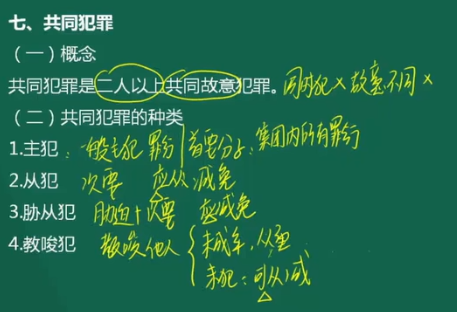
\includegraphics[scale=0.6]{criminal_together}\\ 
\end{frame}

%%%%%%%%%%%%%%%%%%%%%%%%%%%%%%%%%%%%%%%%
% A frame
%%%%%%%%%%%%%%%%%%%%%%%%%%%%%%%%%%%%%%%%
\begin{frame}[t]{刑法}
    
\includegraphics[scale=0.3]{punishment}
    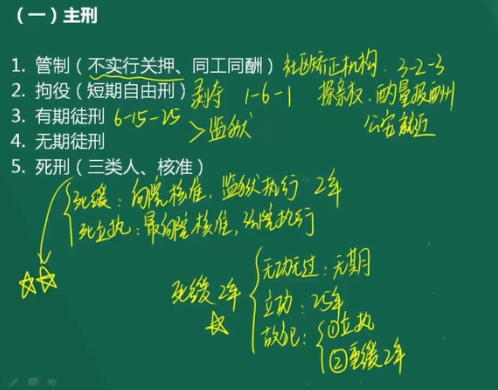
\includegraphics[scale=0.3]{main_punishment}\\
    三类不执行死刑:\textbf{犯罪时未满18}, \textbf{审判时怀孕的妇女} , \textbf{审判时满75, 特别残忍的除外}\\
    判了死缓,不一定会死
    
\end{frame}



%%%%%%%%%%%%%%%%%%%%%%%%%%%%%%%%%%%%%%%%
% A frame
%%%%%%%%%%%%%%%%%%%%%%%%%%%%%%%%%%%%%%%%
\begin{frame}[t]{刑法}
    
\includegraphics[scale=0.6]{accessory_punishment}\\ 
\end{frame}



%%%%%%%%%%%%%%%%%%%%%%%%%%%%%%%%%%%%%%%%
% A frame
%%%%%%%%%%%%%%%%%%%%%%%%%%%%%%%%%%%%%%%%
\begin{frame}[t]{刑法}
    
\includegraphics[scale=0.6]{punishment_practice}\\ 
\end{frame}


%%%%%%%%%%%%%%%%%%%%%%%%%%%%%%%%%%%%%%%%
% A frame
%%%%%%%%%%%%%%%%%%%%%%%%%%%%%%%%%%%%%%%%
\begin{frame}[t]{刑法}
    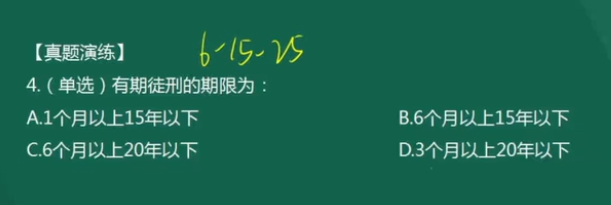
\includegraphics[scale=0.6]{punishment_question}\\ 
\end{frame}


\end{document}
